\documentclass[border=4pt]{standalone}
\usepackage{tikz}
\usetikzlibrary{arrows.meta,positioning,shapes.geometric}
\begin{document}
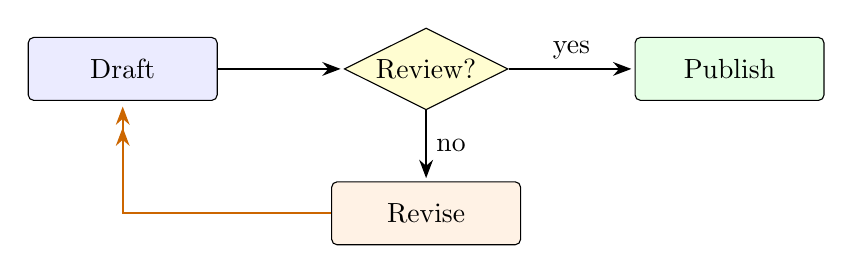
\begin{tikzpicture}[
  node distance=9mm and 16mm,
  block/.style={draw,rounded corners=2pt,minimum width=24mm,minimum height=8mm,align=center},
  decision/.style={draw,diamond,aspect=2,inner sep=1.5pt,align=center},
  flow/.style={line width=.8pt,-{Stealth[sep]}},
  retry/.style={line width=.8pt,orange!80!black,-{Stealth[sep=1pt] Stealth[sep=2pt]}}
]
  \node[block,fill=blue!8] (draft) {Draft};
  \node[decision,fill=yellow!18,right=of draft] (review) {Review?};
  \node[block,fill=green!10,right=of review] (ship) {Publish};
  \node[block,fill=orange!10,below=of review] (revise) {Revise};

  \draw[flow] (draft) -- (review);
  \draw[flow] (review) -- node[above]{yes} (ship);
  \draw[flow] (review) -- node[right]{no} (revise);
  \draw[retry] (revise.west) -| (draft.south);
\end{tikzpicture}
\end{document}
